\begin{figure}[t]
    \centering
    
    \begin{subfigure}[t]{0.48\textwidth}
        \centering
        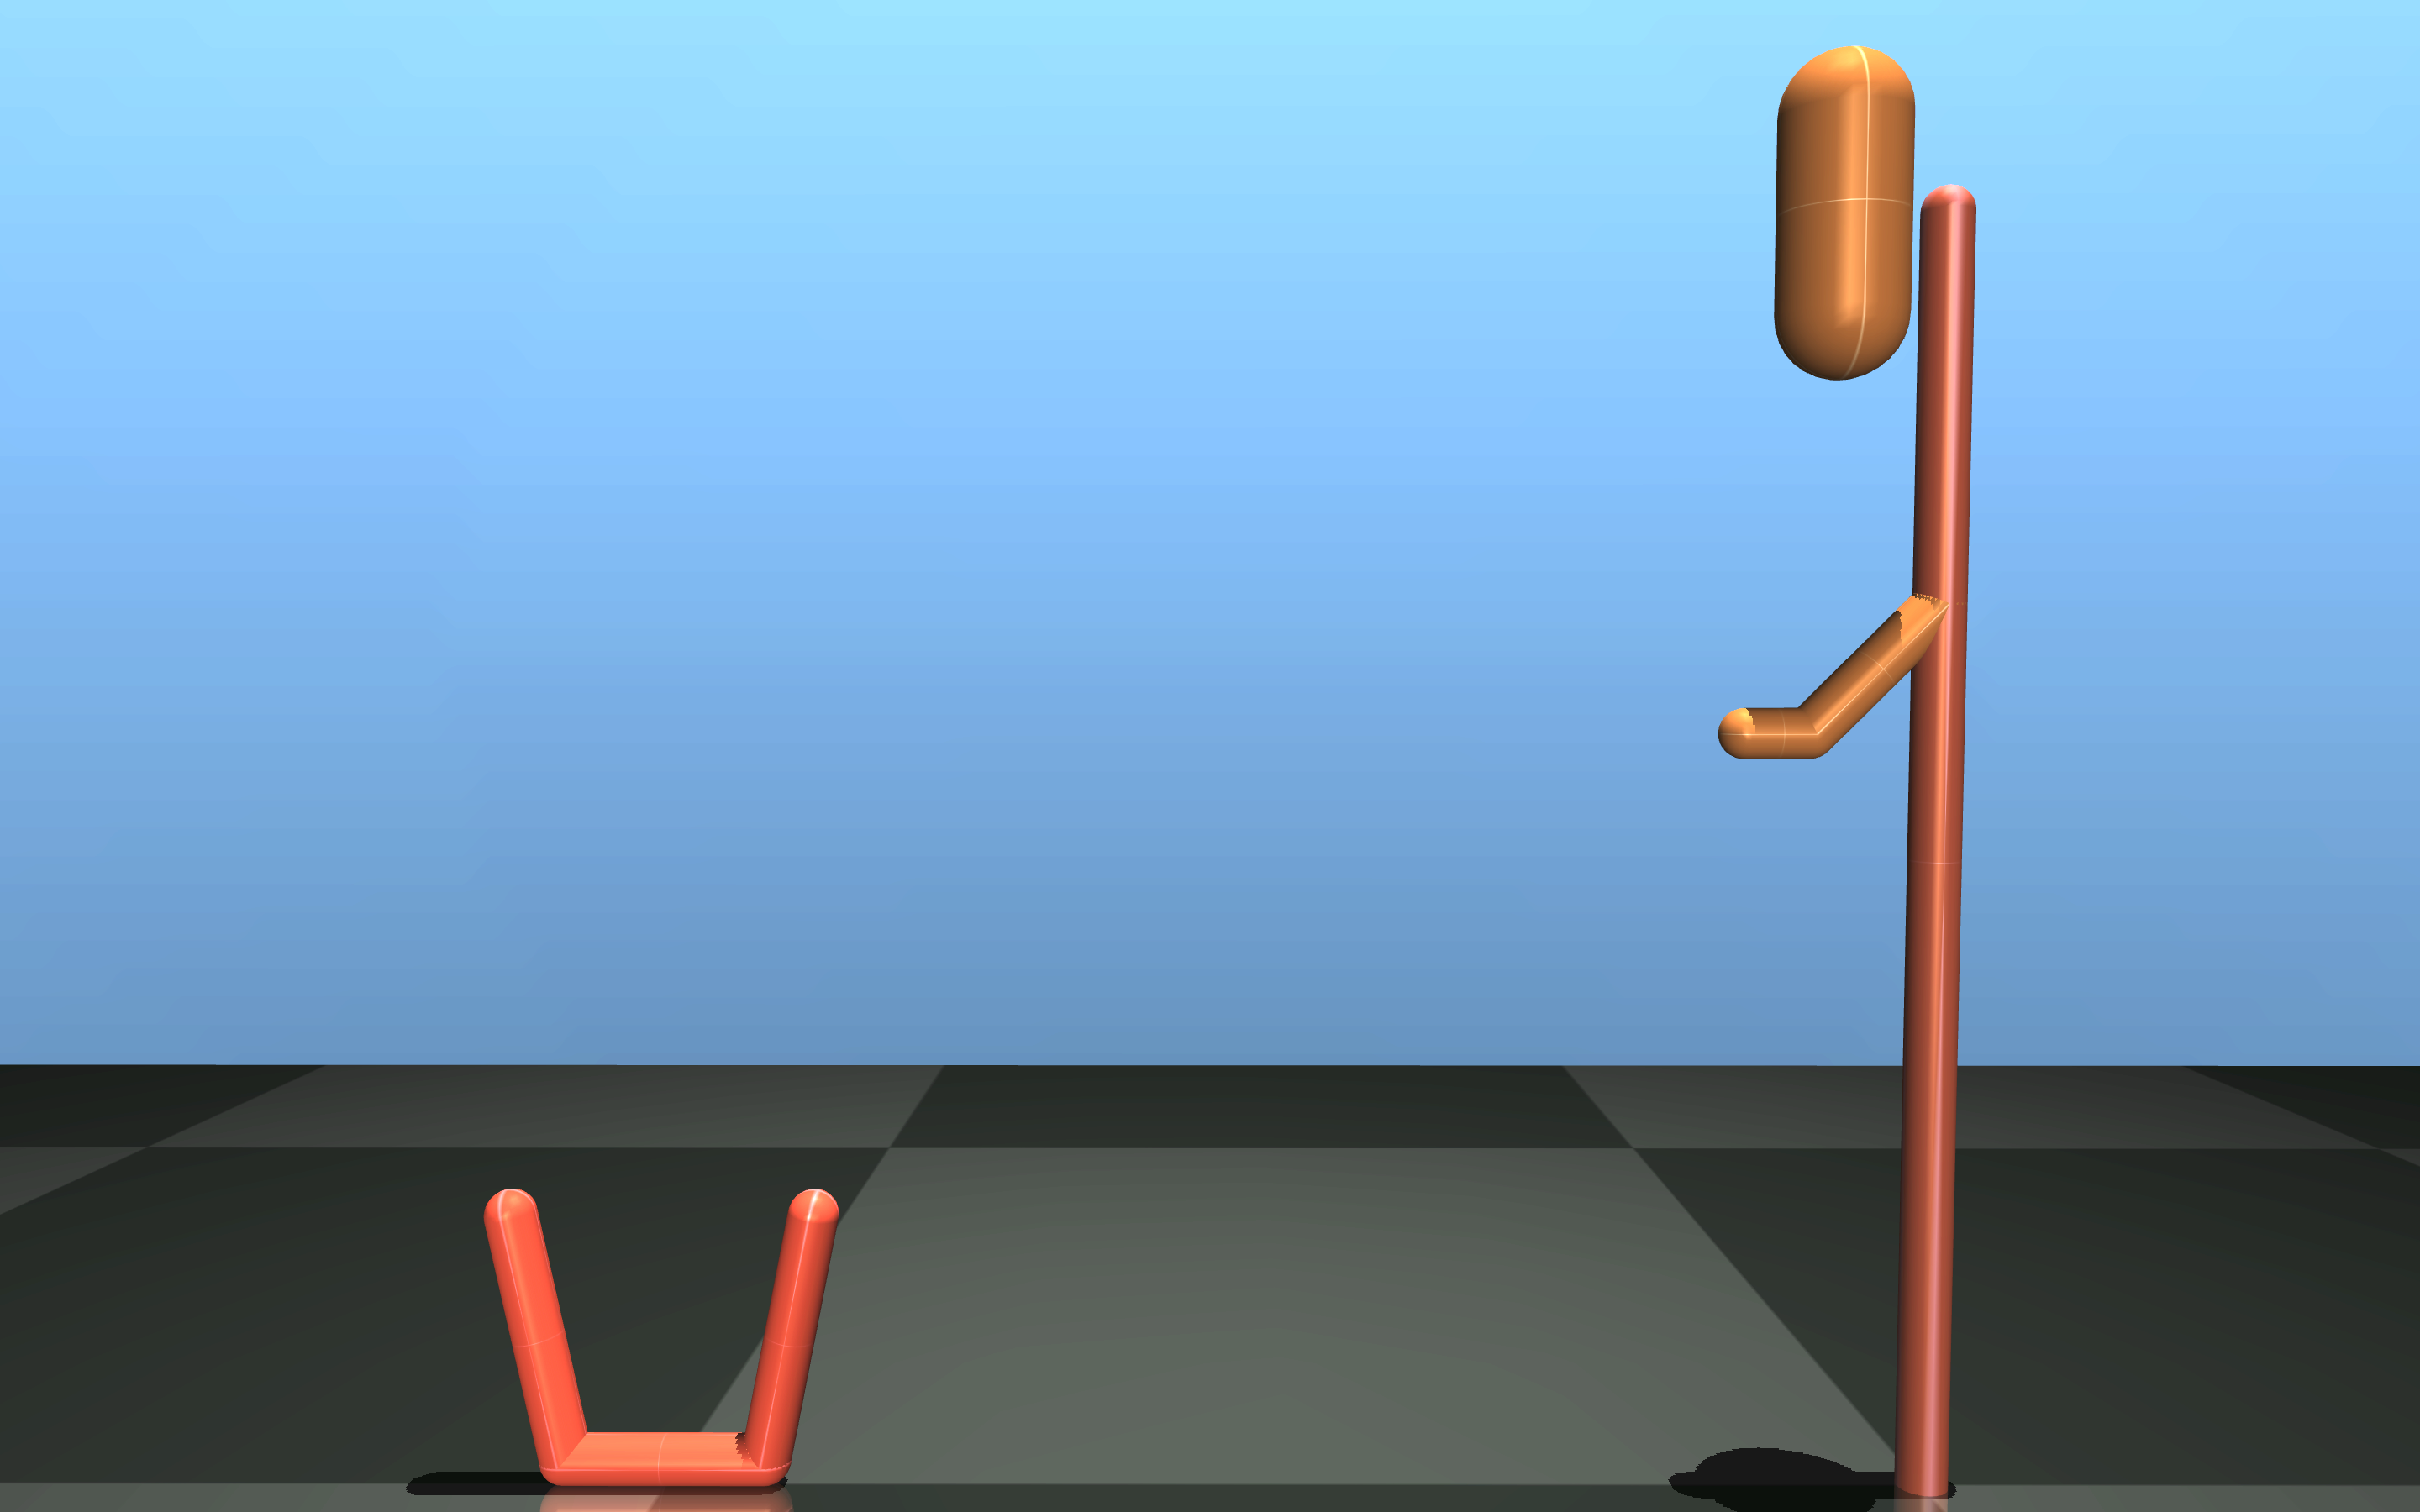
\includegraphics[width=0.24\textwidth]{figures/tosser/tosser1.png}%
        ~%
        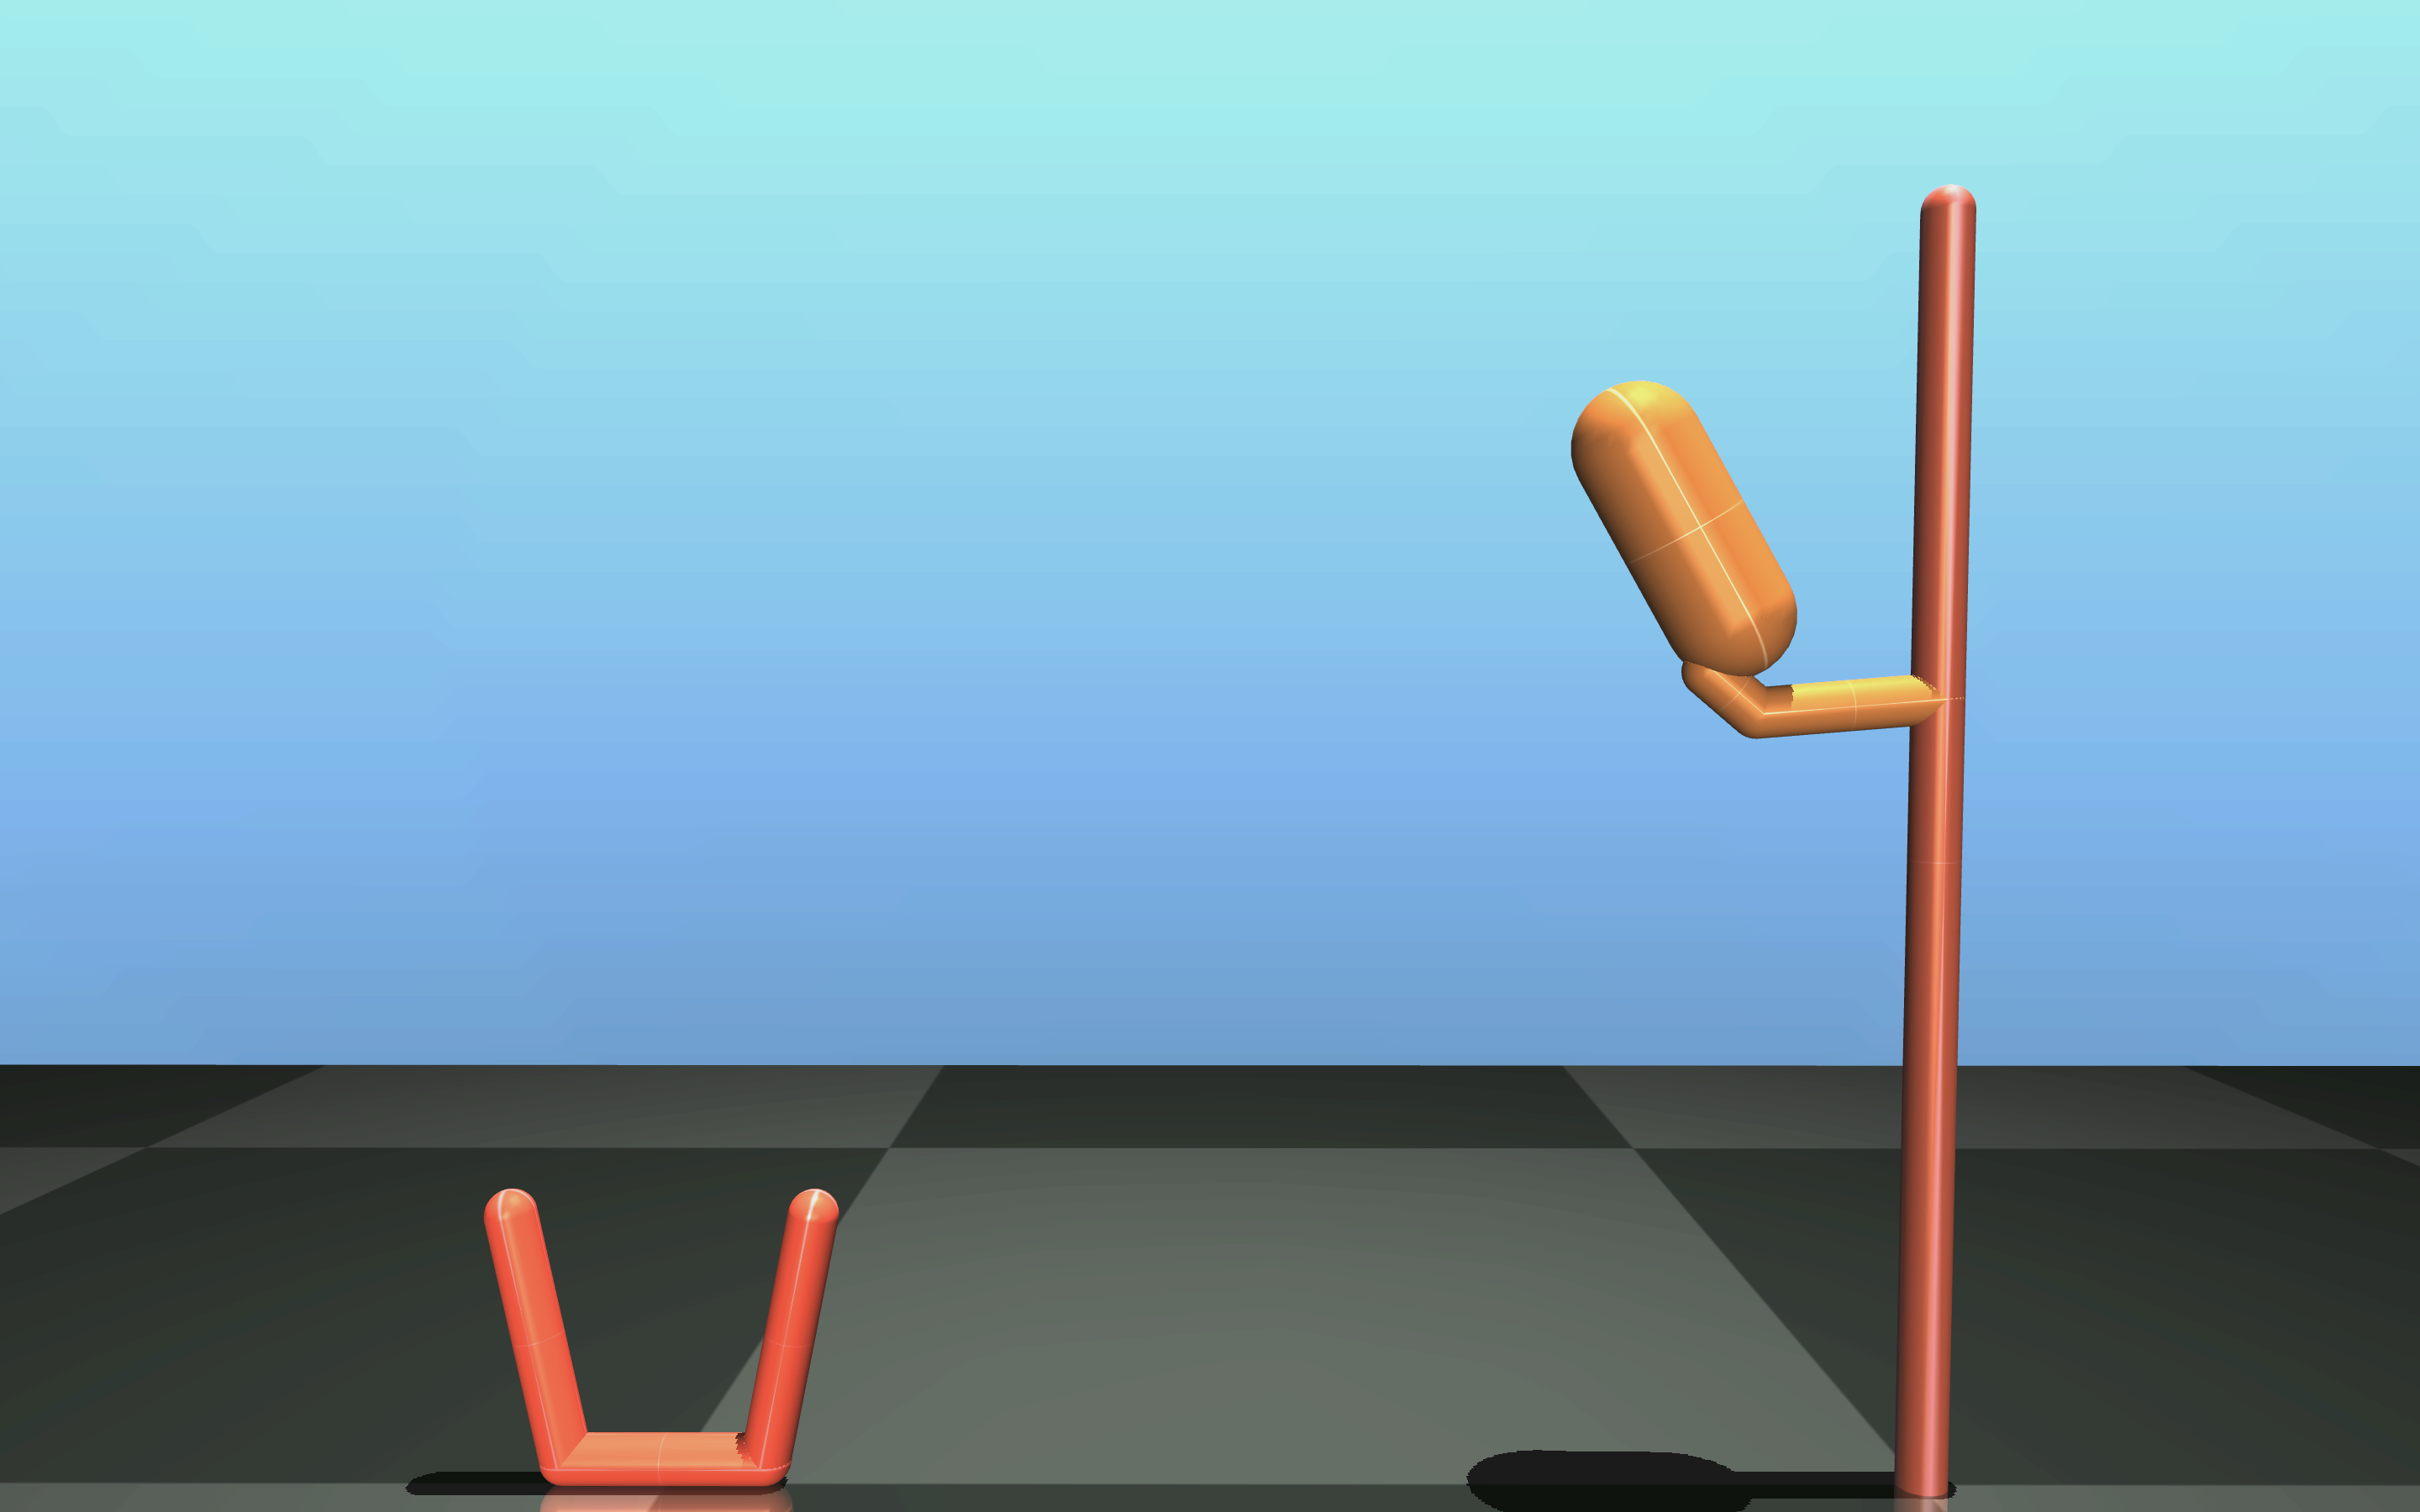
\includegraphics[width=0.24\textwidth]{figures/tosser/tosser2.png}%
        ~%
        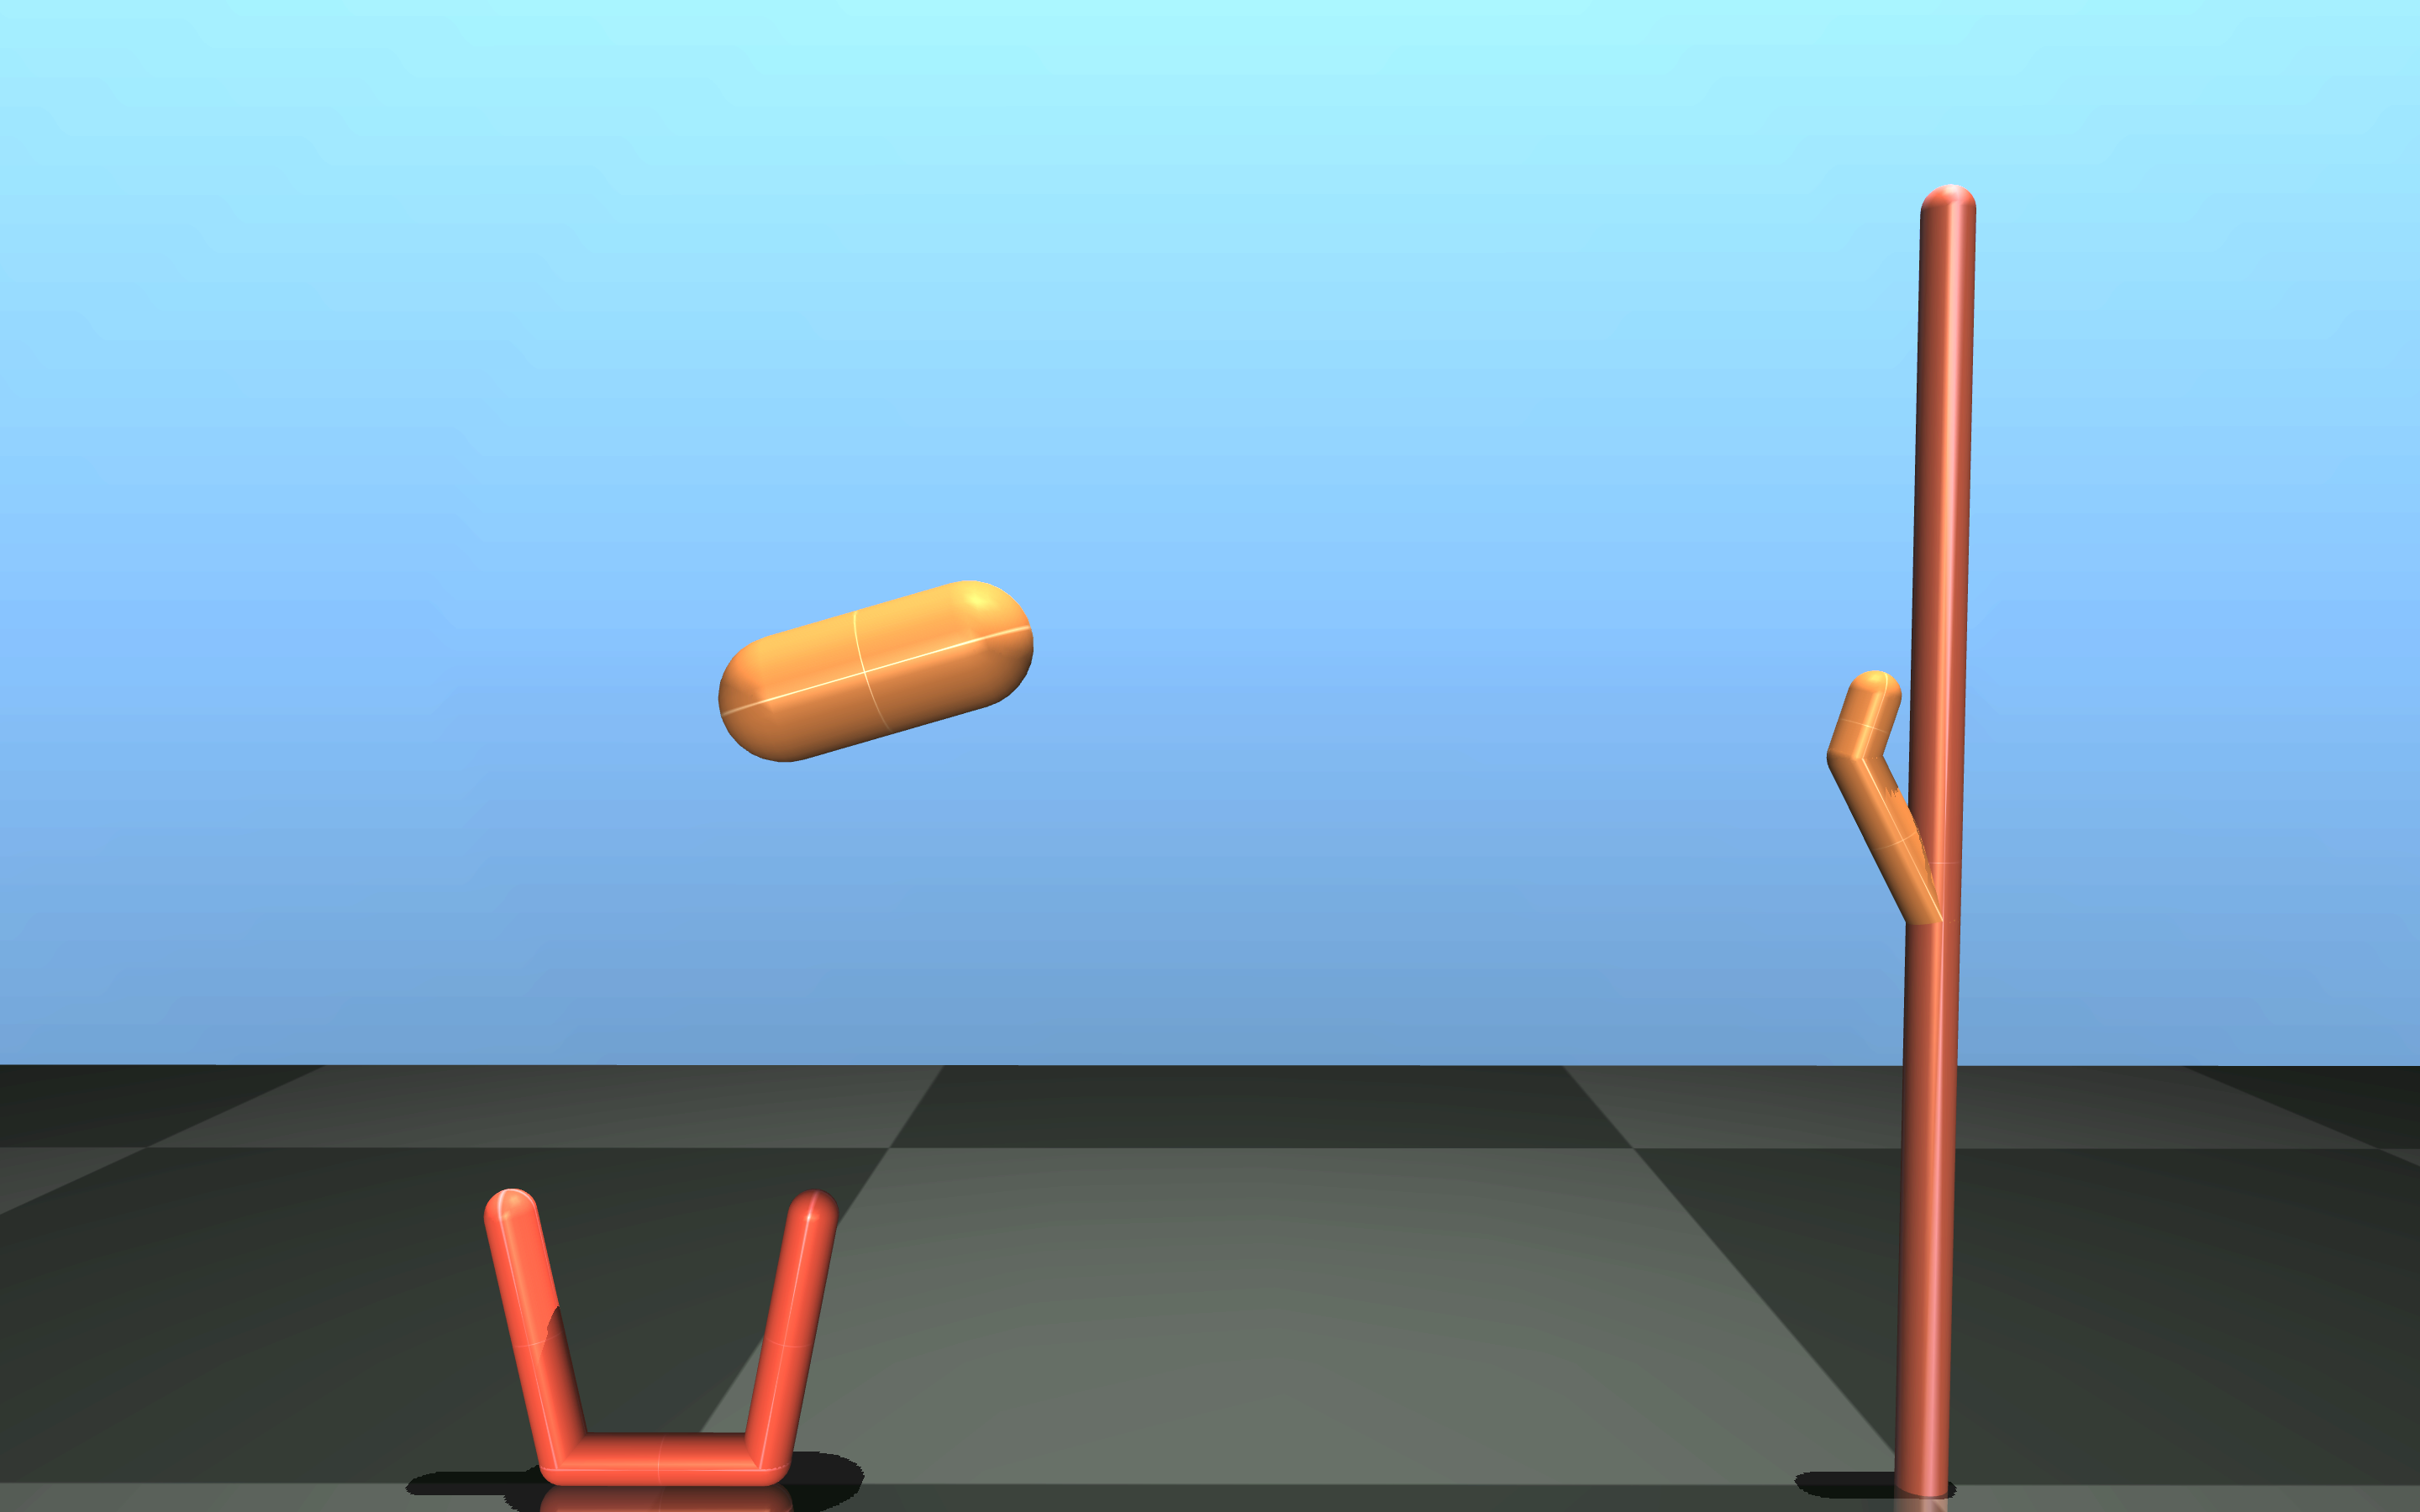
\includegraphics[width=0.24\textwidth]{figures/tosser/tosser3.png}%
        ~%
        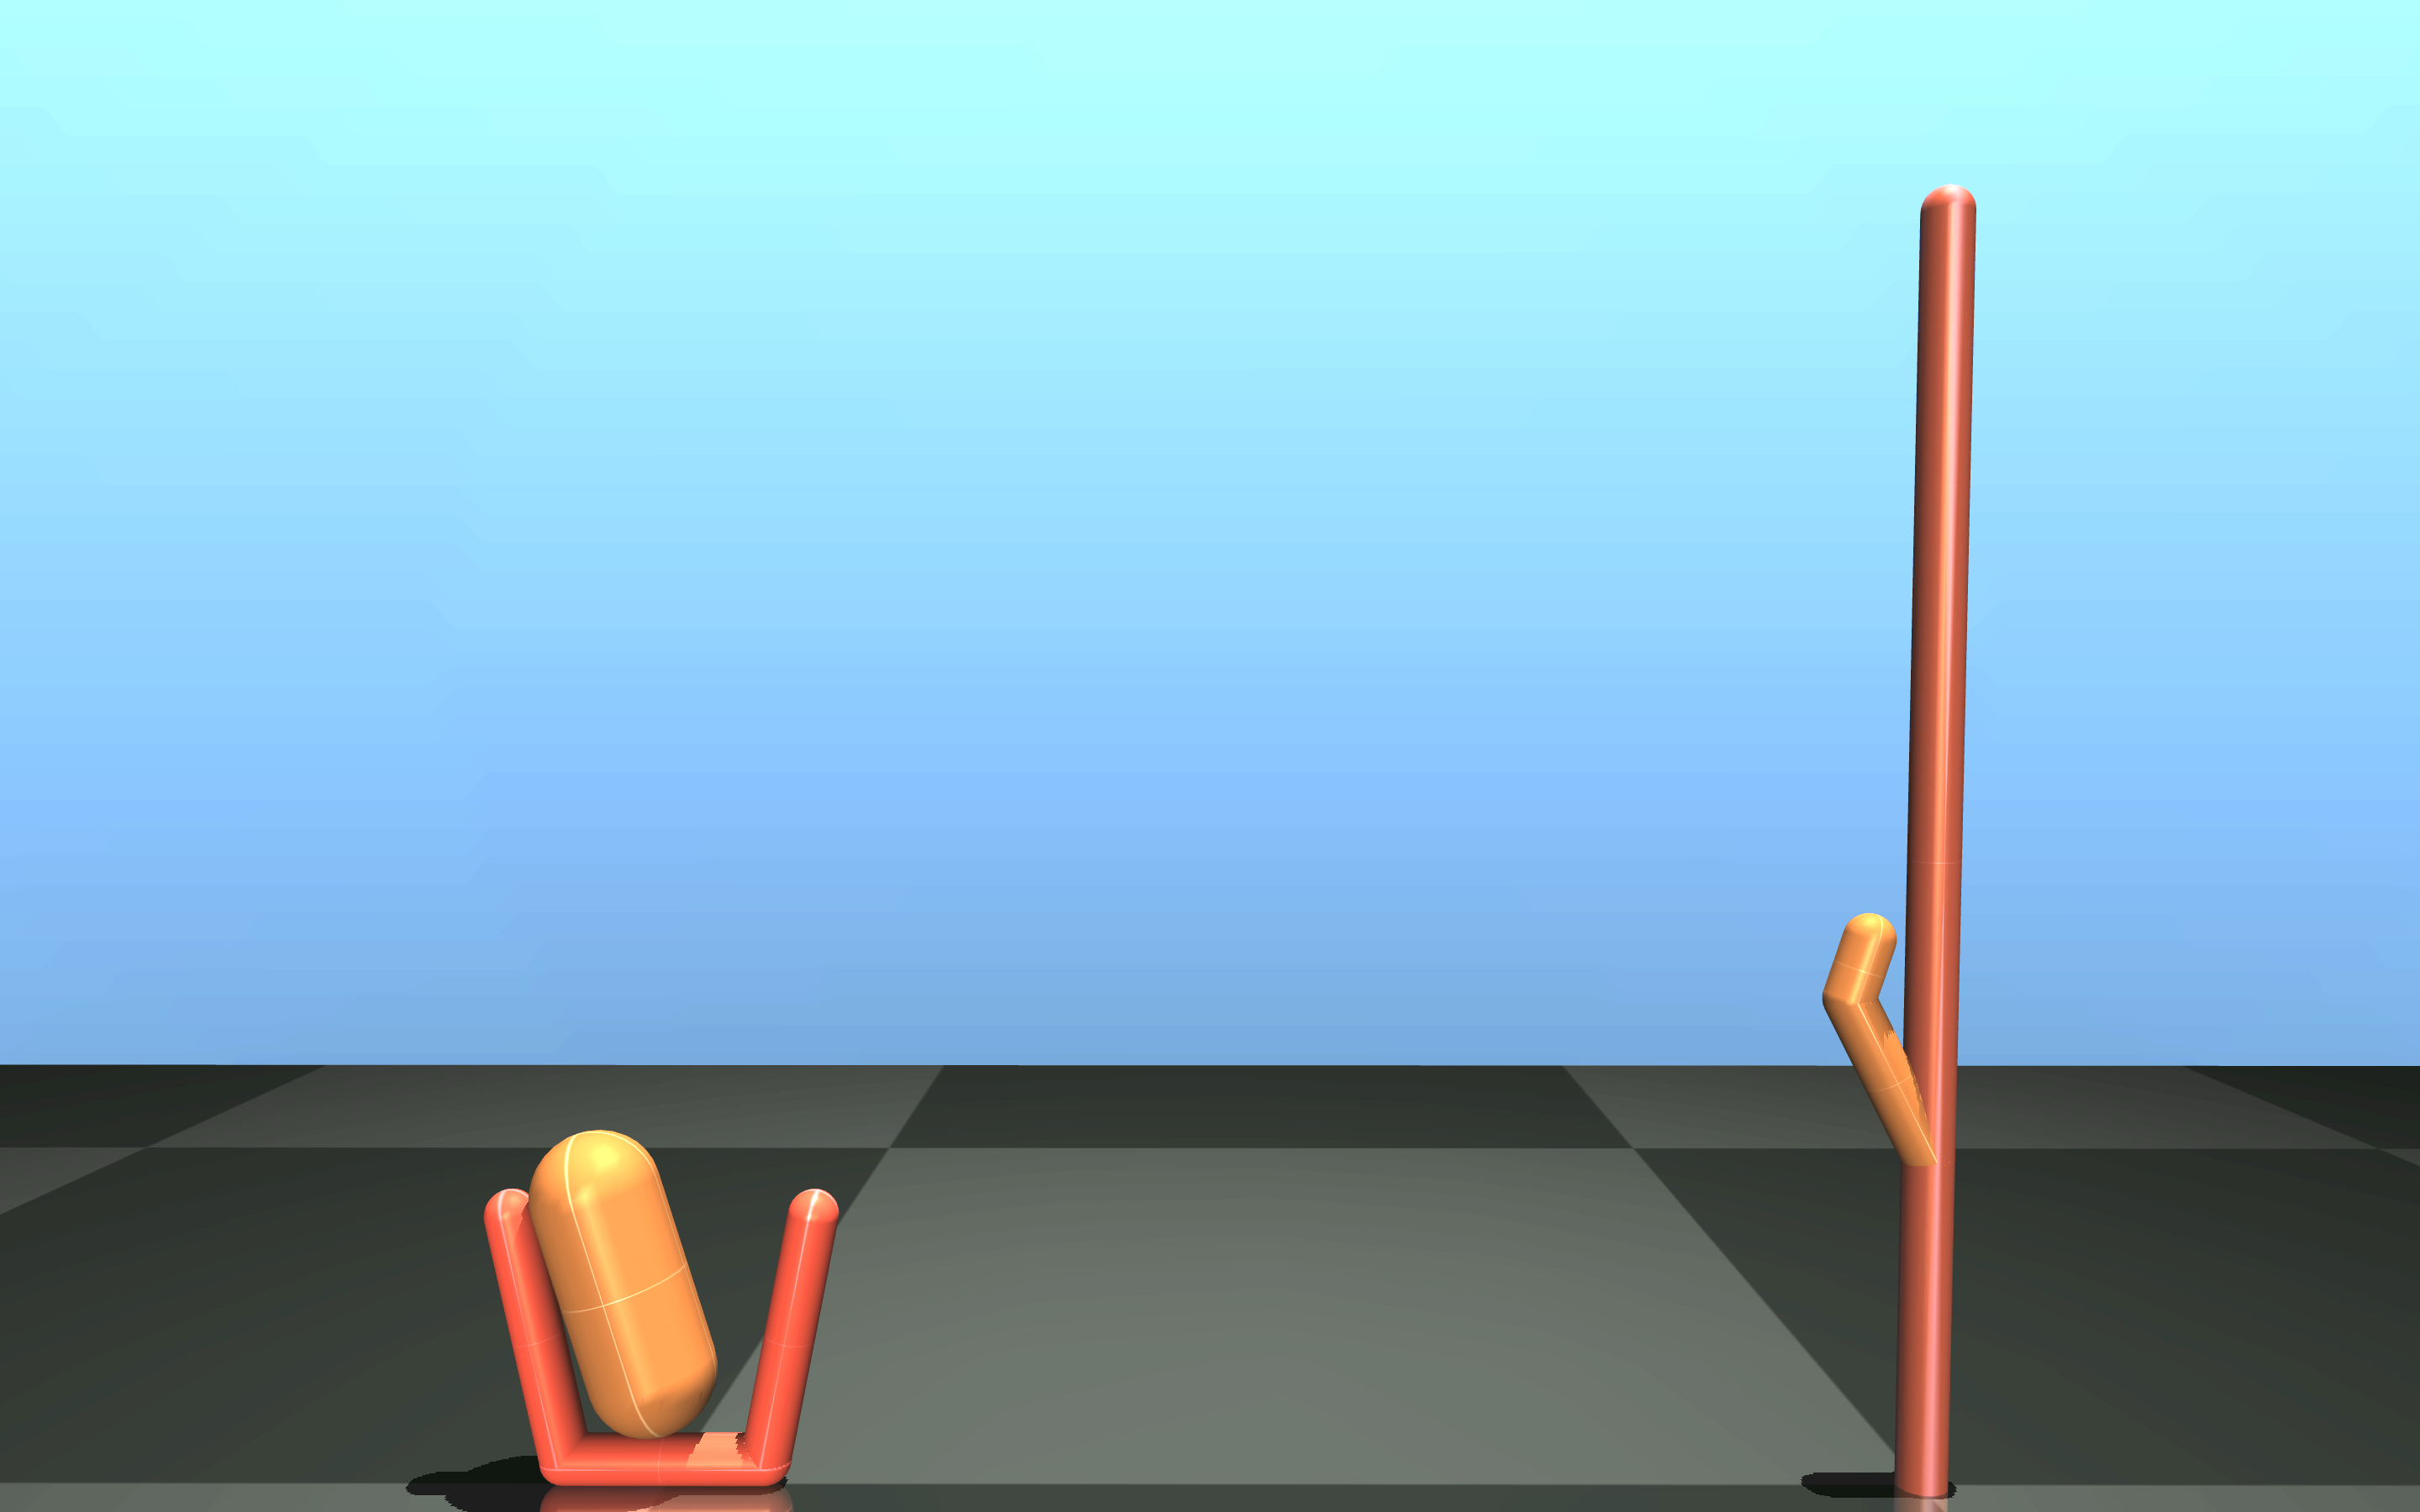
\includegraphics[width=0.24\textwidth]{figures/tosser/tosser4.png}
        \vspace{-0.5cm}
        \caption{ }
        \label{fig:tosser:im}
    \end{subfigure}
    
    % \vspace{-0.2cm}
    \begin{subfigure}[t]{0.24\textwidth}
        \centering
        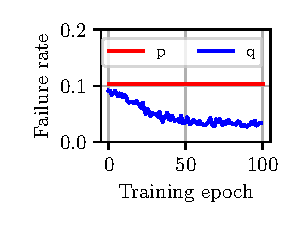
\includegraphics[width=\textwidth]{figures/tosser/TosserNF_cluster_2019_09_28_09_45_55/tosser_nf_bot_rate.pdf}
        \vspace{-0.8cm}
        \caption{ }
        \label{fig:tosser:ar}
    \end{subfigure}%
    ~ 
    \begin{subfigure}[t]{0.24\textwidth}
        \centering
        \includegraphics[width=\textwidth]{figures/tosser/TosserNF_cluster_2019_09_28_09_45_55/tosser_smc_variance_plot.pdf}
        \vspace{-0.8cm}
        \caption{ }
        \label{fig:tosser:smc:var}
    \end{subfigure}
    
    \begin{subfigure}[t]{0.48\textwidth}
        \centering
        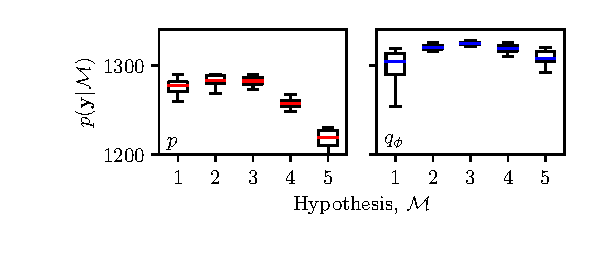
\includegraphics[width=\textwidth]{./figures/tosser/TosserNF_cluster_2019_09_28_09_45_55/tosser_box_plot.pdf}
        % \vspace{-1cm}
        \caption{ }
    \label{fig:tosser_hyp}
    \end{subfigure}
    \vspace{-0.2cm}
    \caption{Results of the ``tosser'' experiment introduced in Section \ref{sec:experiments:tosser}.
    \ref{fig:tosser:im} shows the evolution of state over time.
    \ref{fig:tosser:ar} shows the AF we learn markedly reduces the number of rejections.
    \ref{fig:tosser:smc:var} shows the results of performing SMC using the \emph{a priori} specified proposal and our learned autoregressive flow. 
    The autoregressive flow attains a much lower variance estimate, with a p-value of less than $0.0001$ in a paired t-test, indicating a strong statistical difference in performance.
    \ref{fig:tosser_hyp} shows the results of performing hypothesis testing, where hypothesis $3$ is correct, under a uniform prior over hypothesis. 
    The incorrect hypothesis is selected using $p$, while using $q_{\phi}$ the correct hypothesis is selected, with a statistically significant confidence.
    }
    \label{fig:tosser}
\end{figure}